\documentclass[12pt,a4paper,oneside,ngerman]{article}
\usepackage[utf8]{inputenc}
\usepackage{color}
\usepackage{tikz}
\usepackage{amsmath}
\usepackage{amssymb}
\usepackage{calc}
\usepackage{mathtools}
\usepackage{float}
\usepackage{struktex}
\usepackage{ulem}

\title{EZS}
\author{Simon Krücken}

\newcommand\tab[1][1cm]{\hspace*{#1}}

\begin{document}
    
\begin{titlepage}
%    \maketitle
\end{titlepage}
\tableofcontents
\pagebreak

\section[placeholder]{placeholder}
\section[Zentrale Beschreibegrößen]{Zentrale Beschreibegrößen}
\subsection{placeholder}

\paragraph[Definition]{Definition:}
Realzeitsystem haben neben funktionalen Anforderungen auch \textcolor{red}{zeitliche} Anforderungen.

Ein Realzeitsystem besteht softwaretechnisch aus einer Reihe von Tasks und aus der System-Software.

\begin{figure}[ht]
	\centering
	\includegraphics[scale=0.5]{umlet/rt_control.png}
\end{figure}

\subsubsection{Technischer Prozess}
Rechenzeitanforderung = Ereignis von technischen Prozess
Releasetime = Zeitpunkt des Auftretens der RZ-Anforderung (RZ/RT = Realzeit)

\paragraph[Beispiel]{Beispiel:}
periodisches Signal \textcolor{red}{u} alle 200ms

\fbox{
	\parbox{\textwidth}
	{
		\(t_{Release,u,1}\) = 0ms \(t_{Release,u,2}\) = 200ms \linebreak
		\(t_{Release,u,3}\) = 400ms \(t_{Release,u,4}\) = 600ms \linebreak
						
		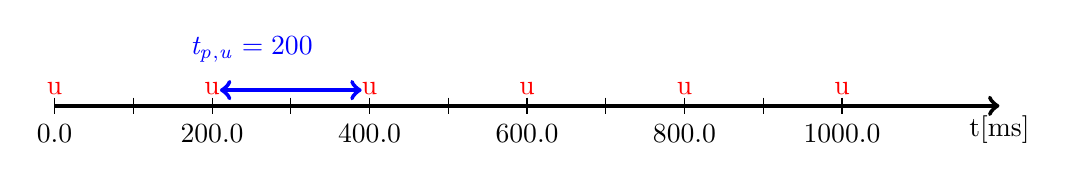
\begin{tikzpicture}
			\draw[ultra thick, ->] (0,0) -- (12,0);
			\draw[ultra thick, <->, draw=blue] (2.1,0.2) -- (3.9,0.2);
			\node[anchor=north] at (2.5,1) {\textcolor{blue}{\(t_{p,u} = 200\)}};
			\node[anchor=north] at (12,0) {t[ms]};
			\foreach \x in {0,1,2,3,4,5,6,7,8,9,10}
			\draw (\x cm,3pt) -- (\x cm,-3pt);
									
			\foreach \x in {0,2,4,6,8,10} {
				\pgfmathsetmacro\result{\x * 100}
				\draw[ultra thick] (\x,0) node[below=3pt,thick] {\result} node[above=3pt] {};
				\draw[ultra thick] (\x,0) node[above] {\textcolor{red}{u}} {};
			}
		\end{tikzpicture}
						
		\textcolor{blue}{Prozesszeit} = zeitlicher Abstand zwischen zwei \textcolor{red}{RZ-Anforderungen} gleichen Typs.
	}
}

\begin{quote}
    \(t_{Pmin,i} = minimal\) =$>$ \(t_{max,i} = \dfrac{1}{ t_{Pmin,i} }\) \\
	\(t_{Pmax,i} = maximal\) \textcolor{gray}{$<$= uninteressant} \\
	\(t_{Dmin,i}\) = minimal zulässige Reaktionszeit \\
	\(t_{Dmax,i}\) = maximal zulässige Reaktionszeit
\end{quote}

Airbag: \\
\(t_{Dmax}\) = 50ms(Zeit bis zum Aufschlag) - 30ms(Zeit zum aufblasen) = 20ms \\
\(t_{Dmin}\) = 0ms

Phase = minimal Zeitlicher Abstand zwischen zwei \textcolor{red}{unterschiedlicher} RZ-Anforderungen \(t_{Ph,i,j}\) \\

\subsubsection{Rechenprozesse}

\begin{description}
\item - Ausführuntgszeit (Executiontime) = Rechenzeit für eine RZ-Anforderung (ohne Warte oder Schlafzeiten)	
	\begin{description}
		\item - WCET \(t_{Emax,i}\) --$>$ Erfahrung oder Messen \textcolor{gray}{Worstcase}
		\item - BCET \(t_{Emin,i}\) = 0 \textcolor{gray}{Bestcase}
	\end{description}
\end{description}

\fbox{
	\parbox{\textwidth}
	{
		\textcolor{red}{ \(t_{E,u}\) = 100ms }
		\textcolor{blue}{ \(t_{E,t}\) = 50ms }
						
		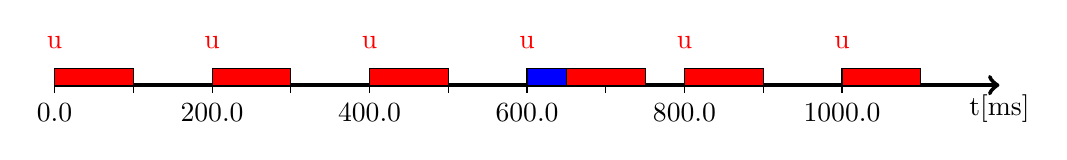
\begin{tikzpicture}
			\draw[ultra thick, ->] (0,0) -- (12,0);
			\node[anchor=north] at (12,0) {t[ms]};
			\foreach \x in {0,1,2,3,4,5,6,7,8,9,10}
			{
				\draw (\x cm,3pt) -- (\x cm,-3pt);
			}

			\foreach \x in {0,2,4,8,10}
			{
				\pgfmathsetmacro\result{\x+1}
				\draw [fill=red] (\x,0) rectangle (\result, 6pt);
			}
			
			\draw [fill=red] (6.5,0) rectangle (7.5, 6pt);
			\draw [fill=blue] (6,0) rectangle (6.5, 6pt);
									
			\foreach \x in {0,2,4,6,8,10} {
				\pgfmathsetmacro\result{\x * 100}
				\draw[ultra thick] (\x,0) node[below=3pt,thick] {\result} node[above=3pt] {};
				\draw[ultra thick] (\x,9pt) node[above] {\textcolor{red}{u}} {};
			}
		\end{tikzpicture}
	}
}

- Reaktionszeit \(t_{R,i}\) = Zeit zwischen dem Auftreten der RZ-Anforderungen \textcolor{red}{i} und dem Ende der Bearbeitung. \\

\(T_{Rmax,i}\) = maximale Reaktionszeit \\
\(T_{Rmin,i}\) = minimale Reaktionszeit \\
\(T_{R,i}\) = \textcolor{red}{\(t_{W,i}\)} \(+ t_{E,i}\) wobei \textcolor{red}{ \(t_{W,i}\) } Summe aller Wartezeiten

\subsubsection{System-software}

- Latenzzeit \(t_{L_i}\) = Zeit zwischen dem Auftreten einer RZ-Anforderung und dem Start der Bearbeitung
\textcolor{blue}{
	- Interrup Latenzzeit
	- Tasklatenzzeit
}

\subsection{Realzeitbedingungen}
\subsubsection{Auslastungsbedingung}

\(\rho_i = \dfrac{t_{E,i}}{t_{P,i}}\) Auslastung dur RZ-Anforderung i \\

\(\rho_{max,i} = \dfrac{t_{Emax,i}}{t_{Pmin,i}}\) Worstcase, max. Auslastung

\fbox{
	\parbox{\textwidth}
	{
		1. RT Bedingung

		\(\rho_{max,ges} = \displaystyle\sum_{j=1}^n \dfrac{t_{Emax,j}}{t_{Pmin,j}} \leq c\) \\
		j = für alle RZ-Anforderungen,
		c = Anzahl der Rechnerkerne
	}
}

\fbox{
	\parbox{\textwidth}
	{
		Beispiel: 2 RZ-Anforderungen A und B

		\begin{equation*}
			\begin{rcases}
				t_{Pmin,A} &= 2ms \\
				t_{Emax,A} &= 0.8ms
			\end{rcases} 
			\text{\(\rho_{max,A} = \dfrac{0.8ms}{2ms} = 0.4ms \)}
		\end{equation*}

		\begin{equation*}
			\begin{rcases}
				t_{Pmin,B} &= 1ms \\
				t_{Emax,B} &= 0.3ms
			\end{rcases} 
			\text{\(\rho_{max,B} = \dfrac{0.3ms}{1ms} = 0.3ms \)}
		\end{equation*}

		\( \rho_{max,ges} = \rho_{max,A} + \rho_{max,B} = 0.7 = 70\% \) \\

		Annahme Singlecore c = 1
		\( \rho_{max,ges} \leq c \) =$>$ \textcolor{green}{\( 0.7 \leq 1\)}

		Auslastungsbedingung erfüllt
	}
}

\subsubsection{Rechtzeitigkeitsbedingung}
Für den Realzeitbetrieb muss die tatsächliche Reaktion innerhalb des Zulässigen Reaktionsbereiches erfolgt sein.

\begin{figure}[ht]
	\centering
	\includegraphics[scale=0.5]{umlet/Rechtzeitigkeitsbedingung.png}
\end{figure}

\fbox{
	\parbox{\textwidth}
	{
		2. RT Bedingung

		Für alle RZ-Anforderungen j muss gelten:

		\( t_{Dmin,j} \leq t_{Rmin,j} \leq t_{Rmax,j} \leq t_{Dmax,j} \)
	}
}

\subsubsection{Harte und weiche Realzeit}

\begin{figure}[H]
	\centering
	\includegraphics[scale=0.4]{umlet/harte_weiche_realzeit.png}
\end{figure}

\subsection{Systemaspekte}
\subsubsection{Unterbrechbarkeit}

\paragraph{Forderung:}
Codesequenzen lassen sich in Teilsequenzen unterteilen, die in korrekter Reihenfolge aber unabhängig voneinander abgearbeitete werden können. \\
=$>$ notwendig für den Realzeitbetrieb

\paragraph{Begründung:}
Ein Messwert soll kontinuierlich erfasst werden. \\
\(t_{Emin,u} = t_{Emax,E} = 0.5ms\) \\
Jeweils 100 Messwerte (alle 100ms) sollen weiterverarbeitet werden \\
\(t_{Pmin,w} = 100ms\) \\
\(t_{Dmin,w} = 0ms\) \\
\(t_{Dmax,w} = 100ms\) \\
\(t_{Dmax,w} = 100ms\) \\ 
\(t_{Emin,w} = t_{Emax,w} = 40ms\) \\

Lösung (ohne Unterbrechbarkeit):\\
\begin{struktogramm}(95,40)
	\while[8]{while(1)}
		\while[7]{100 mal}
			\assign{Messwert einlese / \textcolor{green}{0.5ms}}
		\whileend
		\assign{weiterverarbeiten / \textcolor{green}{40ms}}
	\whileend
\end{struktogramm}

\fbox{
	\parbox{\textwidth}
	{					
		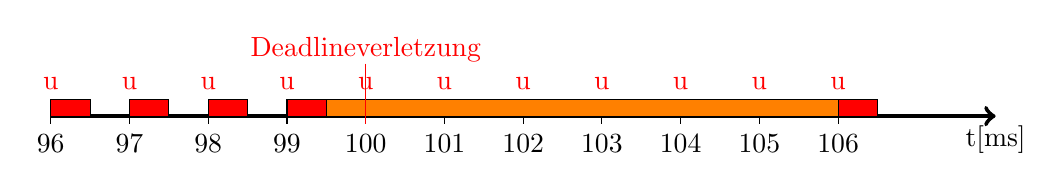
\begin{tikzpicture}
			\draw[ultra thick, ->] (0,0) -- (12,0);
			\node[anchor=north] at (12,0) {t[ms]};
			\foreach \x in {0,...,10}
			\draw (\x cm,3pt) -- (\x cm,-3pt);

			\foreach \x in {0,...,10}
			{
				\pgfmathsetmacro\result{\x+0.5}
				\draw [fill=red] (\x,0) rectangle (\result, 6pt);
			}
			
			\draw [fill=orange] (3.5,0) rectangle (10, 6pt);
			\draw [red](4,19pt) -- (4,-3pt);
			\draw [ultra thick] (4,0) node[above=16pt,thick] {\textcolor{red}{Deadlineverletzung}} {};

									
			\foreach \x in {96,...,106} {
				\pgfmathsetmacro\result{\x-96}
				\draw[ultra thick] (\result,0) node[below=3pt,thick] {\x} node[above=3pt] {};
				\draw[ultra thick] (\result,0) node[above=6pt,thick] {\textcolor{red}{u}} {};
			}
		\end{tikzpicture}
	}
}

\( \rho_{max,u} = \dfrac{0.5ms}{1ms} = 0.5 \);  \(\rho_{max} = \dfrac{40ms}{100ms} = 0.4\) =$>$  \(\rho_{max,ges} = 0.9 \)

Lösung mit Unterbrechbarkeit: \\

\begin{figure}[htb]
	\begin{minipage}[t]{0.4\textwidth}
		\begin{struktogramm}(50,35)
			\while[8]{while(1)}
				\while[7]{100 mal}
					\assign{Messwert einlese / \textcolor{green}{0.5ms}}
				\whileend
				\assign{Thread \textcolor{orange}{W} wecken}
			\whileend
			Thread \textcolor{red}{U}
		\end{struktogramm}%
	\end{minipage}%
	\hfill
	\begin{minipage}[t]{0.4\textwidth}
		\begin{struktogramm}(50,23)
			\while[8]{while(1)}
				\assign{schlafen}
				\assign{weiterverarbeiten}
			\whileend
			Thread \textcolor{orange}{W}
		\end{struktogramm}
	\end{minipage}
\end{figure}

\fbox{
	\parbox{\textwidth}
	{					
		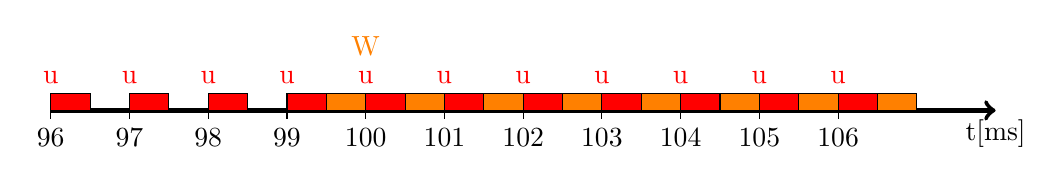
\begin{tikzpicture}
			\draw[ultra thick, ->] (0,0) -- (12,0);
			\node[anchor=north] at (12,0) {t[ms]};
			\foreach \x in {0,...,10}
			\draw (\x cm,3pt) -- (\x cm,-3pt);

			\foreach \x in {0,...,10}
			{
				\pgfmathsetmacro\result{\x+0.5}
				\draw [fill=red] (\x,0) rectangle (\result, 6pt);
			}

			\foreach \x in {3.5,...,10.5}
			{
				\pgfmathsetmacro\result{\x+0.5}
				\draw [fill=orange] (\x,0) rectangle (\result, 6pt);
			}
			
			\draw [ultra thick] (4,0) node[above=16pt,thick] {\textcolor{orange}{W}} {};
						
			\foreach \x in {96,...,106} {
				\pgfmathsetmacro\result{\x-96}
				\draw[ultra thick] (\result,0) node[below=3pt,thick] {\x} node[above=3pt] {};
				\draw[ultra thick] (\result,0) node[above=6pt,thick] {\textcolor{red}{u}} {};
			}
		\end{tikzpicture}
	}
}

\paragraph{Konsequenzen:}
\begin{description}
	\item a) Inter-prozess-Kommunikation (IPC) (Sync, Datenaustausch)
	\item b) Multithreading/Multitasking
\end{description}

\subsubsection{Prioritäten}
\paragraph{Forderung:}
Der Systemarchitekt muss einfluss auf die Abarbeitungsreihenfolge mehrerer Tasks nehmen können z.B. über Prioritäten.

\subsubsection{Ressourcenmanagment}
--$>$ später

\section[System-software]{System-software}
\subsection{Firmware}
\paragraph{Aufgabe:}
\begin{description}
	\item - Basisinitialisierung der Hardware
	\item - Diagnose
	\item - Betriebsinitialisierung
	\item - Laden + Aktivieren von Codes
	\item - Runtime Services
\end{description}
\paragraph{Ausprägungen:}
\begin{description}
	\item - BIOS
	\item - UEFI
	\item - Bootloader ("\textcolor{green}{Das U-Boot}")
	\item - Monitor Software
\end{description}

\subsection{RT-OS}
\paragraph{Definition.:}
Bezeichnung für alle Software-Komponenten, die
\begin{description}
	\item - die Ausführung der Applikationen und
	\item - die Verteilung der Betriebsmittel (Memory, Files, CPU, Drucker, ...) ermöglichen, steuern und überwachen.
\end{description}
\paragraph{Anforderungen:}
\begin{description}
	\item - Zeitverhalten
	\item - Ressourcenverbrauch
	\item - Zuverlässigkeit und Stabilität
	\item - Sicherheit
	\item - Flexibilität und Kompatibilität
	\item - Portierbarkeit
	\item - Skalierbarkeit
\end{description}
\paragraph{Beispiele:}
Sämtliche Betriebsysteme

\begin{figure}[H]
	\paragraph{Systemarchitektur}
	\centering
	\includegraphics[scale=0.5]{umlet/systemarchitektur.png}
\end{figure}

\subsubsection{Systemcall-Interface}
Systemcall = Dienst des Kernels --$>$ 300-400 Dienste

\paragraph{Beispiele:}
open(), close(), read(), write(), exit(), fork(), clone(), clock\_nanosleep(), kill(), adjtime(),...\\
Technische Realisierung: SW-Interrupt

\paragraph{Ablauf:}
ret = write(fd, "Hello World", 13);\\
\textcolor{magenta}{ $\downarrow$ Systemcall "write" per SW-Interrupt}\\
\textcolor{magenta}{"int 0x80", "trap", "sysenter"}\\
\textcolor{magenta}{Systemcall mit EAR = 4} \textcolor{gray}{ $<$-- x86 Register} \\

\textcolor{blue}{ISR (SW-Interrupt 0x80) } \\
\textcolor{blue}{$\downarrow$ EAX = 4 --$>$ bedeutet write } \\
\textcolor{blue}{vfs\_write()} \\
\textcolor{blue}{$\downarrow$ wertet die übrigen CPU-Register aus } \\
\textcolor{blue}{$\downarrow$ fd --$>$ entscheidet über den zu nutzenden Gerätetreiber } \\
\textcolor{blue}{driver\_write() --$>$ gibt Hardwaretehcnisch die Daten aus} \\

\subsubsection{Taskmanagment}
\paragraph{Aufgabe:}
Verwaltung der Ressource CPU
\begin{description}
	\item --$>$ quasi parallele Verarbeitung auf einzelnen CPU-Kernen
	\item --$>$ real parallele Verarbeitung auf Multicore-Rechnern
\end{description}
Scheduling = Auswahl des als nächsten zu bearbeiten Jobs \\
Content Switch = Aktivierung eines Jobs \\

\paragraph{Singelcore-Scheduling}
Realisierung: Modifikation der Rücksprungadresse auf dem Stack beim Interrupt.

\begin{figure}[H]
	\begin{minipage}[t]{6cm}
	\vspace{0pt}
	\centering
	\includegraphics[scale=0.35]{umlet/Singelcore_scheduling.png}
	\end{minipage}
	\hfill
	\begin{minipage}[t]{6cm}
	\vspace{0pt}
	\begin{description}
	\item 1. \textcolor{blue}{Code an der im IP stehenen Adresse wird abgearbeitete}
	\item 2. \textcolor{blue}{IR tritt auf}
		\begin{description}
			\item - Inhalt vom IP wird auf den Stack gelegt
			\item - IP wird auf die Adressee der ISR gelegt (CPU arbeitet die ISR ab)
		\end{description}
	\item 3. \textcolor{blue}{Bei } \textcolor{red}{iret} \textcolor{blue}{ wird die auf dem stack hinterlegte Adressee zurück auf den IP geladen}
	\item --$>$ normale Verarbeitung wird fortgesetzt
	\end{description}
	\end{minipage}

	\textcolor{orange}{* zusätlicher Code der die auf dem Stack liegende Adresse ändert} \\
	\textcolor{orange}{z.B. die} \textcolor{green}{1000} \textcolor{orange} {wird mit} 4000 \textcolor{orange}{überschrieben} \\
\end{figure}


\begin{figure}[H]
	\fbox{
		\parbox{\textwidth}
		{					
			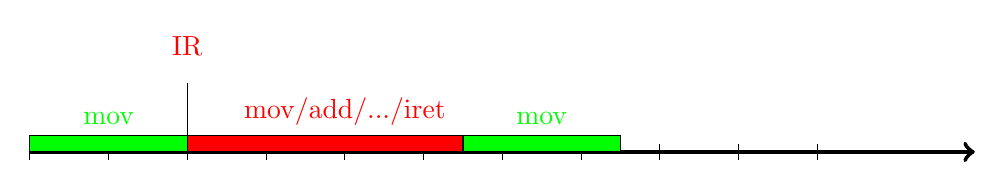
\begin{tikzpicture}
				\draw[ultra thick, ->] (0,0) -- (12,0);
				\foreach \x in {0,...,10}
				\draw (\x cm,3pt) -- (\x cm,-3pt);

				\draw [fill=green] (0,0) rectangle (2, 6pt);
				\draw [fill=red] (2,0) rectangle (5.5, 6pt);
				\draw [fill=green] (5.5,0) rectangle (7.5, 6pt);
				
				\draw (2,25pt) -- (2,-3pt);
				\draw[ultra thick] (2,25pt) node[above=6pt,thick] {\textcolor{red}{IR}} {};

				\draw[ultra thick] (1,0) node[above=6pt,thick] {\textcolor{green}{mov}} {};

				\draw[ultra thick] (4,0) node[above=6pt,thick] {\textcolor{red}{mov/add/.../iret}} {};

				\draw[ultra thick] (6.5,0) node[above=6pt,thick] {\textcolor{green}{mov}} {};

			\end{tikzpicture}
		}
	}

	\fbox{
		\parbox{\textwidth}
		{					
			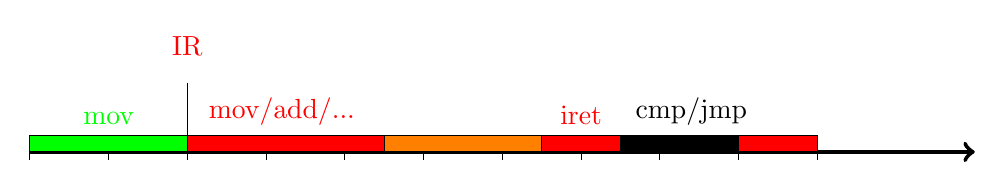
\begin{tikzpicture}
				\draw[ultra thick, ->] (0,0) -- (12,0);
				\foreach \x in {0,...,10}
				\draw (\x cm,3pt) -- (\x cm,-3pt);

				\draw [fill=green] (0,0) rectangle (2, 6pt);
				\draw [fill=red] (2,0) rectangle (4.5, 6pt);
				\draw [fill=orange] (4.5,0) rectangle (6.5, 6pt);
				\draw [fill=red] (6.5,0) rectangle (7.5, 6pt);
				\draw [fill=black] (7.5,0) rectangle (9, 6pt);
				\draw [fill=red] (9,0) rectangle (10, 6pt);
				
				\draw (2,25pt) -- (2,-3pt);
				\draw[ultra thick] (2,25pt) node[above=6pt,thick] {\textcolor{red}{IR}} {};

				\draw[ultra thick] (1,0) node[above=6pt,thick] {\textcolor{green}{mov}} {};
				\draw[ultra thick] (3.2,0) node[above=6pt,thick] {\textcolor{red}{mov/add/...}} {};
				\draw[ultra thick] (7,0) node[above=6pt,thick] {\textcolor{red}{iret}} {};
				\draw[ultra thick] (8.4,0) node[above=6pt,thick] {\textcolor{black}{cmp/jmp}} {};

			\end{tikzpicture}
		}
	}
\end{figure}

Eine Datenstruktur wird benötigt, um alle Informationen zu einer Codesequenzen speichern(Job, Rechenprozess): \textcolor{blue}{Task Controll Block (TCB)}

\begin{figure}[H]
	\centering
	\includegraphics[scale=0.5]{umlet/TCB.png}
\end{figure}

\begin{figure}[H]
	\centering
	\includegraphics[scale=0.8]{umlet/taskzustand.png}
\end{figure}

\paragraph{Erzeugen von Rechenprozessen}
Neue Jobs werden durch Kopieren von
\begin{description}
	\item - TCB
	\item - Stack-Segment
	\item - Code-Segment
	\item - Daten Segment
	\item - Neue PID vergeben
\end{description}
erzeugt

\begin{figure}[H]
	\centering
	\includegraphics[scale=0.8]{umlet/fork.png}
\end{figure}

\begin{figure}[H]
	\centering
	\includegraphics[scale=0.8]{umlet/clone.png}
\end{figure}

Threads einer Threadgruppe teilen sich Code- und Datensegment
Vorteil:
\begin{description}
	\item - Speicherplatzersparnis
	\item - schnell erzeugt
	\item - einfache IPC (Inter Process Communication)
\end{description}
Nachteil:
\begin{description}
	\item - Safety: Ein amok laufender Thread bringt die gesamte Threadgruppe in einen inkonsistenten Zustand.
\end{description}

\subsubsection{Scheduling}
\paragraph{Def.:}
Auswahl der Task, der arbeiten/rechnen darf \\
\emph{Content Switch:} Aktivierung der ausgewählten Task \\
\emph{Statisches Scheduling:} Bedarfsituation ist bekannt \\
\rotatebox[origin=c]{180}{$\Lsh$} Reihenfolge (Plan) kann im vorhinein festgelegt werden (SPS)\\
\emph{Dynamisches Scheduling:} Die Auswahl erfolgt auf Basis der aktuellen Bedarfsituation (z.B. PC, Smartphone)\\
\emph{Singlecore Scheduling:} Quasiparallele Verarbeitung auf einem CPU-Kern\\
\emph{Multicore Scheduling:} Realparallele Verarbeitung auf mehrerern CPU-Kernen\\
\rotatebox[origin=c]{180}{$\Lsh$} Verteilungsaufgabe
\emph{Preemption Point:} Auftreten einer RF-Anforderung --$>$ Interrup Serivce Routine(ISR) wird aktiv --$>$ Scheduling

\subsubsection{Singlecore Scheduling}
\begin{table}[H]
	\caption{Beispieldaten:}
	\begin{tabular}{|l|l|l|l|l|l|}
	\hline
	RZ-Anf & \(t_{Pmin}\) & \(t_{Dmin}\) & \(t_{Dmax}\) & \(t_{Emin}\) & \(t_{Emax}\) \\ \hline
	\textcolor{red}{v}      & 20ms         & 0ms          & 20ms         & 1ms          & 5ms          \\ \hline
	\textcolor{blue}{g}      & 40ms         & 0ms          & 40ms         & 1ms          & 15ms         \\ \hline
	\textcolor{green}{u}      & 30ms         & 0ms          & 30ms         & 1ms          & 10ms         \\ \hline
	\end{tabular}
\end{table}

\emph{First come First Serve (FCFS, FIFO)} \\
\begin{description}
	\item - Lauffähige Jobs werden gemäß Auftrittszeitpunkt in eine Queue eingeführt
	\item - Der erste Job in der Liste wird ausgewählt
	\item - Er darf solange die CPU benutzen (rechnen) bis
	\begin{description}
		\item a) er sich schlafen legt
		\item b) er sich beendet
	\end{description}
	\item Ein "aufgeweckter" Job wird an den Anfang der Queue gestelt und unterbricht den laufenden Job nicht.
\end{description}


\fbox{
	\parbox{\textwidth}
	{					
		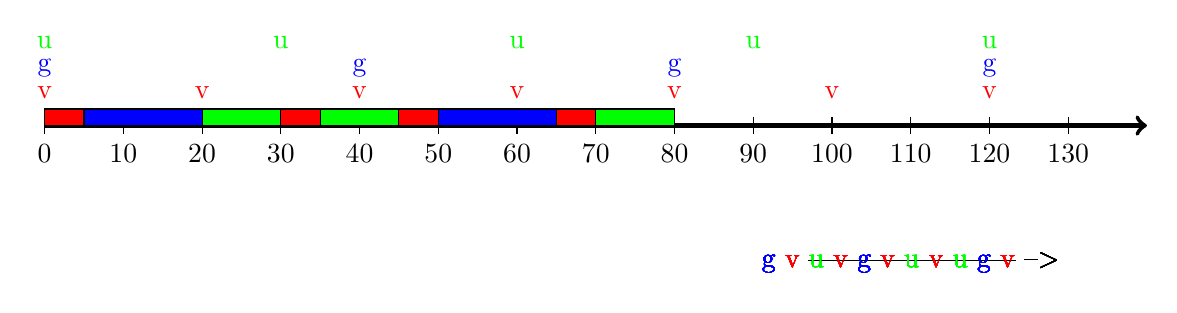
\begin{tikzpicture}
			\draw[ultra thick, ->] (0,0) -- (14,0);
			\foreach \x in {0,...,13}
			\draw (\x cm,3pt) -- (\x cm,-3pt);


			\draw [fill=red] (0,0) rectangle (0.5, 6pt);
			\draw [fill=blue] (0.5,0) rectangle (2, 6pt);
			\draw [fill=green] (2,0) rectangle (3, 6pt);
			\draw [fill=red] (3,0) rectangle (3.5, 6pt);
			\draw [fill=green] (3.5,0) rectangle (4.5, 6pt);
			\draw [fill=red] (4.5,0) rectangle (5, 6pt);
			\draw [fill=blue] (5,0) rectangle (6.5, 6pt);
			\draw [fill=red] (6.5,0) rectangle (7, 6pt);
			\draw [fill=green] (7,0) rectangle (8, 6pt);
		

			\foreach \x in {0,2,...,12}
			{
				\draw[ultra thick] (\x,0) node[above=6pt,thick] {\textcolor{red}{v}} {};
			}

			\foreach \x in {0,4,...,12}
			{
				\draw[ultra thick] (\x,0) node[above=14pt,thick] {\textcolor{blue}{g}} {};
			}

			\foreach \x in {0,3,...,12}
			{
				\draw[ultra thick] (\x,0) node[above=24pt,thick] {\textcolor{green}{u}} {};
			}

			\foreach \x in {0,...,13} {
			\pgfmathtruncatemacro\result{round(\x * 10)}
			\draw[ultra thick] (\x,0) node[below=3pt,thick] {\result} node[above=3pt] {};


			\draw[ultra thick] (11,-2) node[above,thick] {
			\textcolor{blue}{g}
			\textcolor{red}{v}
			\sout{\textcolor{green}{u}
			\textcolor{red}{v}
			\textcolor{blue}{g}
			\textcolor{red}{v}
			\textcolor{green}{u}
			\textcolor{red}{v}
			\textcolor{green}{u}
			\textcolor{blue}{g}
			\textcolor{red}{v}}
			--$>$} {};

		}
		\end{tikzpicture}
	}
}

\emph{Zeitscheibenverfahren (Round Robin, Rate Monotonic)}
\begin{description}
	\item - Lauffähige Jobs werden gemäß Auftrittszeitpunkt in eine Queue eingehängt
	\item - Der erste Job in der Liste wird ausgewählt
	\item - Er darf die CPU benutzen bis
	\begin{description}
		\item a) er sich schlafen left
		\item b) er sich beendet
		\item c) seine Zeitscheibe (Quantum) aufgebraucht ist
	\end{description}
	\item - Ein aufgeweckter Job wird ans Ende der Queue angehängt
\end{description}
\textcolor{magenta}{Zeitscheibe 10ms}

\fbox{
	\parbox{\textwidth}
	{					
		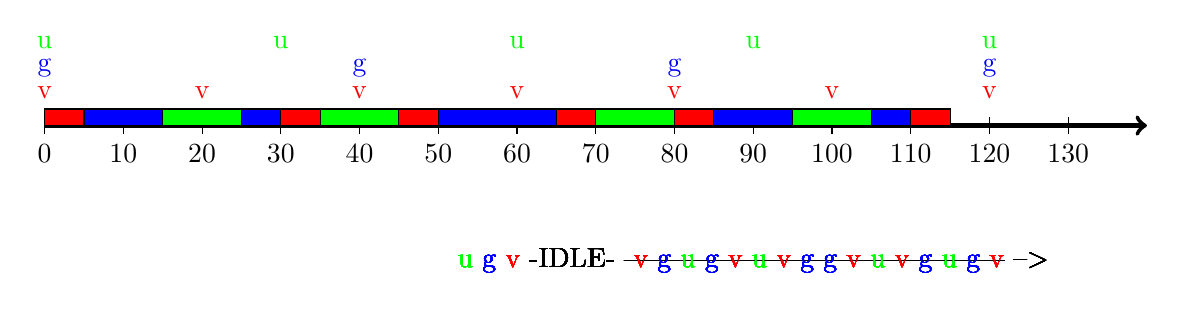
\begin{tikzpicture}
			\draw[ultra thick, ->] (0,0) -- (14,0);
			\foreach \x in {0,...,13}
			\draw (\x cm,3pt) -- (\x cm,-3pt);

			\draw [fill=red] (0,0) rectangle (0.5, 6pt);
			\draw [fill=blue] (0.5,0) rectangle (1.5, 6pt);
			\draw [fill=green] (1.5,0) rectangle (2.5, 6pt);
			\draw [fill=blue] (2.5,0) rectangle (3, 6pt);
			\draw [fill=red] (3,0) rectangle (3.5, 6pt);
			\draw [fill=green] (3.5,0) rectangle (4.5, 6pt);
			\draw [fill=red] (4.5,0) rectangle (5, 6pt);
			\draw [fill=blue] (5,0) rectangle (6.5, 6pt);
			\draw [fill=red] (6.5,0) rectangle (7, 6pt);
			\draw [fill=green] (7,0) rectangle (8, 6pt);
			\draw [fill=red] (8,0) rectangle (8.5, 6pt);
			\draw [fill=blue] (8.5,0) rectangle (9.5, 6pt);
			\draw [fill=green] (9.5,0) rectangle (10.5, 6pt);
			\draw [fill=blue] (10.5,0) rectangle (11, 6pt);
			\draw [fill=red] (11,0) rectangle (11.5, 6pt);
		

			\foreach \x in {0,2,...,12}
			{
				\draw[ultra thick] (\x,0) node[above=6pt,thick] {\textcolor{red}{v}} {};
			}

			\foreach \x in {0,4,...,12}
			{
				\draw[ultra thick] (\x,0) node[above=14pt,thick] {\textcolor{blue}{g}} {};
			}

			\foreach \x in {0,3,...,12}
			{
				\draw[ultra thick] (\x,0) node[above=24pt,thick] {\textcolor{green}{u}} {};
			}

			\foreach \x in {0,...,13} {
			\pgfmathtruncatemacro\result{round(\x * 10)}
			\draw[ultra thick] (\x,0) node[below=3pt,thick] {\result} node[above=3pt] {};


			\draw[ultra thick] (9,-2) node[above,thick] {

			\textcolor{green}{u}
			\textcolor{blue}{g}
			\textcolor{red}{v}
			-IDLE-
			\sout{ \textcolor{red}{v}
			\textcolor{blue}{g}
			\textcolor{green}{u}
			\textcolor{blue}{g}
			\textcolor{red}{v}
			\textcolor{green}{u}
			\textcolor{red}{v}
			\textcolor{blue}{g}
			\textcolor{blue}{g}
			\textcolor{red}{v}
			\textcolor{green}{u}
			\textcolor{red}{v}
			\textcolor{blue}{g}
			\textcolor{green}{u}
			\textcolor{blue}{g}
			\textcolor{red}{v}}
			--$>$} {};
		}
		\end{tikzpicture}
	}
}

\emph{Prioritätengesteuertes Scheduling}
\begin{description}
	\item - Jedem Job wird eine Priorität zugewiesen
	\item - Der \textcolor{magenta}{Lauffähige} Job mit der höchsten Priorität wird ausgewählt
	\item - Er darf rechnen bis
	\begin{description}
		\item a) er sich schlafen legt
		\item b) er sich beendet
		\item c) ein Job mit höherer Prio Lauffähig wird
	\end{description}
\end{description}
\textcolor{blue}{Problem: Verteilung der Prioritäten}

\fbox{
	\parbox{\textwidth}
	{	
		kurze \(t_{Emax}\) \textcolor{red}{und} kurze \(t_{Pmin}\) --$>$ hohe Prio
	}
}

\textcolor{red}{Gibt es zwischen \(t_{E,i}\) und \(t_{P,i}\) keine Korrelation hilft bei der Prioritätenverteilung nur ausprobieren!} \\

\paragraph{Beispiel:}
	\textcolor{red}{V = 1 (höchste Prio)} \\
	\textcolor{blue}{G = 3 (niedrigste Prio)} \\
	\textcolor{green}{U = 2 (mittlere Prio)} \\


\fbox{
	\parbox{\textwidth}
	{					
		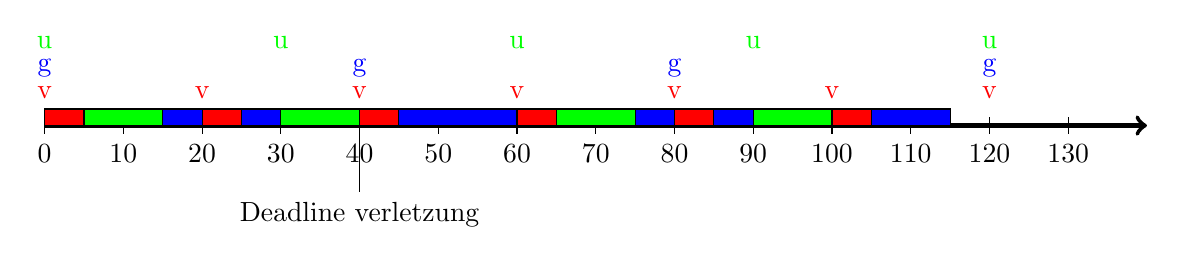
\begin{tikzpicture}
			\draw[ultra thick, ->] (0,0) -- (14,0);
			\foreach \x in {0,...,13}
			\draw (\x cm,3pt) -- (\x cm,-3pt);

			\draw [fill=red] (0,0) rectangle (0.5, 6pt);
			\draw [fill=green] (0.5,0) rectangle (1.5, 6pt);
			\draw [fill=blue] (1.5,0) rectangle (2, 6pt);
			\draw [fill=red] (2,0) rectangle (2.5, 6pt);
			\draw [fill=blue] (2.5,0) rectangle (3, 6pt);
			\draw [fill=green] (3,0) rectangle (4, 6pt);
			\draw [fill=red] (4,0) rectangle (4.5, 6pt);
			\draw [fill=blue] (4.5,0) rectangle (6, 6pt);
			\draw [fill=red] (6,0) rectangle (6.5, 6pt);
			\draw [fill=green] (6.5,0) rectangle (7.5, 6pt);
			\draw [fill=blue] (7.5,0) rectangle (8, 6pt);
			\draw [fill=red] (8,0) rectangle (8.5, 6pt);
			\draw [fill=blue] (8.5,0) rectangle (9, 6pt);
			\draw [fill=green] (9,0) rectangle (10, 6pt);
			\draw [fill=red] (10,0) rectangle (10.5, 6pt);
			\draw [fill=blue] (10.5,0) rectangle (11.5, 6pt);

			\foreach \x in {0,2,...,12}
			{
				\draw[ultra thick] (\x,0) node[above=6pt,thick] {\textcolor{red}{v}} {};
			}

			\foreach \x in {0,4,...,12}
			{
				\draw[ultra thick] (\x,0) node[above=14pt,thick] {\textcolor{blue}{g}} {};
			}

			\foreach \x in {0,3,...,12}
			{
				\draw[ultra thick] (\x,0) node[above=24pt,thick] {\textcolor{green}{u}} {};
			}

			\draw (4 ,3pt) -- (4 ,-24pt);
			\draw[ultra thick] (4,0) node[below=24pt,thick] {Deadline verletzung} node[above=3pt] {};

			\foreach \x in {0,...,13} {
			\pgfmathtruncatemacro\result{round(\x * 10)}
			\draw[ultra thick] (\x,0) node[below=3pt,thick] {\result} node[above=3pt] {};

		}
		\end{tikzpicture}
		\textcolor{blue}{g} tritt erneut auf obwohl \textcolor{blue}{g} noch nicht fertig abgearbeitet ist.
		Die letzten 5ms vom alten \textcolor{blue}{g} werden erst bei 45ms abgearbeitet.
	}
}

\emph{Deadline-Scheduling (Earliest Deadline First)}
\begin{description}
	\item - Der Lauffähige Job, der als erstes fertig sein muss (\(t_{Dmax}\)) darf rechnen.
	\item - Er darf arbeiten bis
	\begin{description}
		\item a) er sich schlafen legt
		\item b) er sich beendet
		\item c) ein Job Lauffähig wird, der früher abgeschlossen sein muss.
	\end{description}
\end{description}

\fbox{
	\parbox{\textwidth}
	{					
		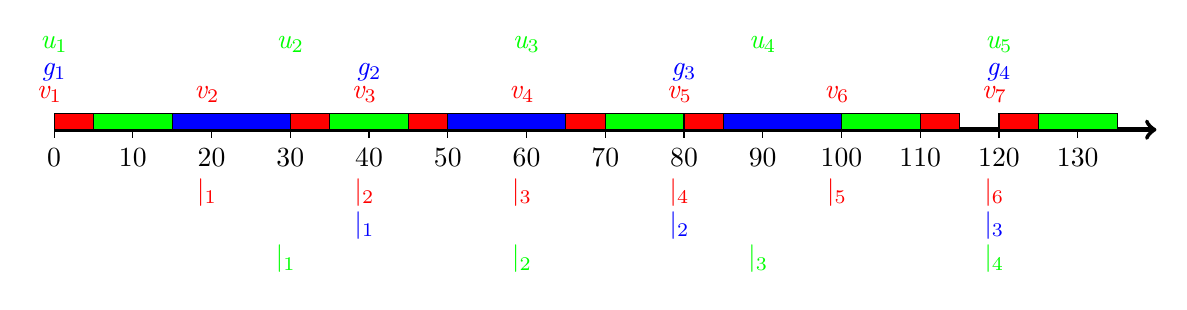
\begin{tikzpicture}
			\draw[ultra thick, ->] (0,0) -- (14,0);
			\foreach \x in {0,...,13}
			\draw (\x cm,3pt) -- (\x cm,-3pt);

			\draw [fill=red] (0,0) rectangle (0.5, 6pt);
			\draw [fill=green] (0.5,0) rectangle (1.5, 6pt);
			\draw [fill=blue] (1.5,0) rectangle (3, 6pt);
			\draw [fill=red] (3,0) rectangle (3.5, 6pt);
			\draw [fill=green] (3.5,0) rectangle (4.5, 6pt);
			\draw [fill=red] (4.5,0) rectangle (5, 6pt);
			\draw [fill=blue] (5,0) rectangle (6.5, 6pt);
			\draw [fill=red] (6.5,0) rectangle (7, 6pt);
			\draw [fill=green] (7,0) rectangle (8, 6pt);
			\draw [fill=red] (8,0) rectangle (8.5, 6pt);
			\draw [fill=blue] (8.5,0) rectangle (10, 6pt);
			\draw [fill=green] (10,0) rectangle (11, 6pt);
			\draw [fill=red] (11,0) rectangle (11.5, 6pt);
			\draw [fill=red] (12,0) rectangle (12.5, 6pt);
			\draw [fill=green] (12.5,0) rectangle (13.5, 6pt);


			\foreach \x in {0,2,...,12}
			{
				\pgfmathtruncatemacro\result{round((\x / 2)+1}
				\pgfmathtruncatemacro\resutt{\x + 2}
				\draw[ultra thick] (\x,0) node[above=6pt,thick] {\textcolor{red}{ \( v_\result \) }} {};
				\ifnum\x<12
					\draw[ultra thick] (\resutt,0) node[below=14pt,thick] {\textcolor{red}{ \( |_\result \) }} {};
				\fi
			}

			\foreach \x in {0,4,...,12}
			{
				\pgfmathtruncatemacro\result{round((\x / 4)+1}
				\pgfmathtruncatemacro\resutt{\x + 4}
				\draw[ultra thick] (\x,0) node[above=14pt,thick] {\textcolor{blue}{\( g_\result \)}} {};
				\ifnum\x<12
					\draw[ultra thick] (\resutt,0) node[below=26pt,thick] {\textcolor{blue}{ \( |_\result \) }} {};
				\fi
			}

			\foreach \x in {0,3,...,12}
			{
				\pgfmathtruncatemacro\result{round((\x / 3)+1}
				\pgfmathtruncatemacro\resutt{\x + 3}
				\draw[ultra thick] (\x,0) node[above=24pt,thick] {\textcolor{green}{\( u_\result \)}} {};
				\ifnum\x<12
					\draw[ultra thick] (\resutt,0) node[below=38pt,thick] {\textcolor{green}{ \( |_\result \) }} {};
				\fi
			}

			\foreach \x in {0,...,13} {
			\pgfmathtruncatemacro\result{round(\x * 10)}
			\draw[ultra thick] (\x,0) node[below=3pt,thick] {\result} node[above=3pt] {};
			}
		\end{tikzpicture}
	}
}

Eignung für RT-Systeme: \textcolor{orange}{optimales Verfahren}\\

\emph{Kombinierte Schedulingverfahren}
\begin{description}
	\item - Prioritätengesteuertes Scheduling --$>$ Prioritätsebene
	\item - Jobs mit gleiche Priorität (=auf gleicher Prioritätsebene)
	\begin{equation*}
		\begin{rcases}
				werden \textcolor{white}{a} gemaess \textcolor{white}{a} a) Round Robin\\
				\textcolor{white}{werden gemaessaai } b) FCFS (FIFO)
		\end{rcases} 
		\text{ \textcolor{magenta}{Posix-Scheduling}}
	\end{equation*}
	\item gescheduled \textcolor{green}{=$>$ Linux,} \textcolor{magenta}{{ \[\underbrace{VxWorks, Windows}_{\text{Round Robin}} \]}}
\end{description}

\begin{figure}[H]
	\centering
	\includegraphics[scale=0.5]{umlet/windows_prio.png}
\end{figure}

\paragraph{Linux:}
Prioritäten per Konsole vergeben: \textcolor{green}{chrt 69 ./carrera} // werte von 0..99 \\
Konzept der Scheduling Klassen:
\begin{description}
	\item 0 Stop-Sched-Class
	\item 1 Prioritäten gesteuertes Scheduling
	\item 2 EDF (Earliest Deadline first)
	\item 3 CFS (Completly Fair Scheduling)
	\item 4 Idle Shed. Class
\end{description}

\subsubsection{Multicore Scheduling}
\paragraph{Aufgabe:}
Verteilung der Jobs auf die CPU-Kerne, so dass unsere Zeitbedingunen eingehalten werden \emph{und} das System (eneregie-)effizient arbeitet.

\paragraph{Lösungen:}
\begin{description}
	\item 1. Partitioniert Scheduling\\ Tasks werden auf die CPU-Kerne Statisch verteilt.(per Hand)
	\item 2. Semipartioniertes Scheduling\\ tastk werden in Gruppen auf die CPU-Kerne verteilt.
	\item 3. Globales Scheduling\\ Scheduler verteilt die Tasks auf Basis der aktuellen Lastsituation.
\end{description}

\emph{Taskmigration:} Verschiebung von Tasks auf andere CPU-Kerne\\
Problemstellung:
\begin{description}
	\item - \textcolor{green}{Kosten} der Taskmigration sind abhängig von der eingesetzten Hardware
	\item - \textcolor{green}{Nutzen} ist abhängig von der eingesetzten Hardware
\end{description}

\emph{Hardware-Architekturen}
SMP: Symmetirc Multi Processing (= alle CPU Kerne sind gleich)\\
Kosten: mittel\\
Nutzen: mittel\\
SMT: Symmetric Multi Threading (Hyperthreading, = Verdopplung der Instruction Pipeline)\\
Kosten: niedrig\\
Nutzen: niedrig\\
NUMA: Non Uniform memory Architecture\\
Kosten: hoch\\
Nutzen: hoch\\

\begin{figure}[H]
	\centering
	\includegraphics[scale=0.4]{umlet/numa.png}
\end{figure}

bigLITTLE-Architektur: (z.B. 4(starke) + 4(schwache) Kerne) \\
Optimierungsziel: Energieeffizienz\\
Kosten(in hinblick auf Leistung) = SMP(mittel)\\
Nutzen = SMP(mittel)\\

AMP: Asymmetirc Multiprocessing (unterschiedliche CPU-Kerne)\\
Kosten: hoch\\
Nutzen: je nach Anwendung\\
=$>$ wird in der Praxis über Partitioniertes Scheduling genutzt.

\begin{figure}[H]
	\centering
	\includegraphics[scale=0.4]{umlet/numa_node.png}
\end{figure}

\begin{figure}[H]
	Linux bildet beim Booten eine \textcolor{orange}{Scheduling Domain}
	\centering
	\includegraphics[scale=0.6]{umlet/scheduling_domain.png}
\end{figure}

Der Multicore Scheduler balanziert die last innerhalb einer Scheduling Domain --$>$ sorgt für ausgeglichene Lastverhältnisse.\\
Die einzelnen Cores verwenden einen Singlecore Scheduler.
Unter Linux ist der name der Rechenprozesse, die für Multicore-Scheduling zuständig sind "\textcolor{magenta}{migration}".\\
\paragraph{Der Multicore Scheduler wird aktiv:}
\begin{description}
	\item - exit()
	\item - pthread\_create(), clone(), fork()
	\item - clock\_nanosleep()
	\item - zeitgesteuert
\end{description}

\subsubsection{Memory Managment}
\paragraph{Aufgaben:}
\begin{description}
	\item - Speicherschutz
	\item - Adressumsetzung
	\item - virtuellen Speicher zur verfügung stellen
	\item - erweiterten Speicher zur verfügung stellen
\end{description}
Technologien:
\begin{description}
	\item 1. Segmentierung
	\item 2. Paging (Seitenorientierung)
\end{description}

\begin{figure}[ht]
	\emph{Segmentierung}
	\centering
	\includegraphics[scale=0.8]{umlet/Seite_30.png}
\end{figure}

\begin{figure}[ht]
	\centering
	\includegraphics[scale=0.8]{umlet/Paging.png}
\end{figure}

Auf 32 Bit Systemen: Two Level Paging\\
Auf 64 Bit Systemen: Three Level paging\\

\paragraph{Konsequenz:}
Um eine Variable aus dem Hauptspeicher zu lesen, sind auf einem 32 Bit System 3 Hauptspeicherzugriffe notwendig.\\
=$>$ zur Optimierung TCB (Cache)\\
Außerdem: In den Page Directories sind die obersten Einträge (auf 32Bit 15 Byte) für den Kernelspace reserviert.

\subsubsection{I/O Managment}

\begin{figure}[H]
	\begin{minipage}[t]{6cm}
	\vspace{0pt}
	Aufgabe:
	\begin{description}
	\item a) Einheitliche API für den HW Zugriff
	\item b) Systemkonforme Integration von Hardware über Gerätetreiber
	\item c) Strukturierter Zugriff auf Daten (Filesystem)
	\end{description}
	\end{minipage}
	\hfill
	\begin{minipage}[t]{6cm}
		\vspace{0pt}
		\centering
		\includegraphics[scale=0.35]{umlet/userland_kernel.png}
	\end{minipage}
\end{figure}

API: \textcolor{blue}{open, cloes(), read(), write(), ioctl(), fcntl(), seek()}

\fbox{
	\parbox{\textwidth}
	{	
		\emph{Hintergrund: Direct I/O - Bufferd I/O}\\
		\textcolor{red}{printf("$\backslash$n Hallo");} $<$-- Buffered\\
		\textcolor{green}{printf("Hallo $\backslash$n");}

		Buffered I/O =$>$ Daten werden aus Performance-Gründen zwischengespeichert.
		Reale Ausgabe erfolgt, wenn der Zwischenspeicher (Buffer) voll ist oder wenn ein "$\backslash$n" kommt.\\

		\textcolor{green}{fopen(), fclose(), fprintf(), fwrite(), fread(), fflush()}\\

		Direct I/O =$>$ Ein-/Ausgabe-Aufrufe werden direkt ausgeführt.
	}
}

\emph{Kontrollfluss (Wann?, Unter welchen Umständen?)}\\
\paragraph{Zugriffsarten:}
\begin{description}
	\item - Blockierend
	\item - nicht Blockierend
	\item - Asynchron
\end{description}

a) Blockierend\\
Beispiel "read": Job schläft, bis die angeforderten Daten zur Verfügungn stehen --$>$ Carrear Bahn, eigene Spur\\

b) Nicht Blockierend \textcolor{blue}{fd = open("dev/carrera", O\_RDWR$|$O\_NONBLOCK)} \\
Beispiel "read": Job bekommt die angeforderten Daten oder die Information, dass zu Zeit des Aufrufes keine Daten zur Verfügung stehen.\\
--$>$ Job wird nicht schlafen gelegt.

c) Asynchron\\
Aufträge werden dem Kernel übergeben und das Resultat zu einem späteren zeitpunkt abgeholt.\\

\emph{Systemkonforme Integration von Hardware über Gerätetreiber}\\
\paragraph{Idee:}
open, close, read, write, ... bieten einen einheitlichen Zugriff auf unterschiedliche Peripherie
\paragraph{Außerdem:}
Applikationen sollen keinesfalls direkt auf Peripherie zugreifen können (Safety)
\paragraph{Und:}
Applikationen sollen keine Details der Hardware (z.B. Adressen, Bitmaskierungen, Gerätetreiber) kennen müssen.

\begin{figure}[ht]
	\centering
	\includegraphics[scale=0.5]{umlet/Seite_34.png}
\end{figure}

\emph{Filesysteme}
Strukturen zur Ablage von Daten auf Hintergrundspeicher in hierarchisch organisierten Dateien.\\
\paragraph{Beispiel:} Ext4, NTFS, FAT32, exFat, JFFS2, ISO9660, ...\\

\paragraph{Merkmale:}
\begin{description}
	\item - maximale FileSystem-Größe
	\item - Anzahl Dateien
	\item - maximale Datei Größe
	\item - Attribute
	\item - Zugriffszeit
\end{description}

\end{document}